% details-of-test-conditions.tex

\chapter{Propulsion Interpolation Scheme}

\begin{figure}
\centering
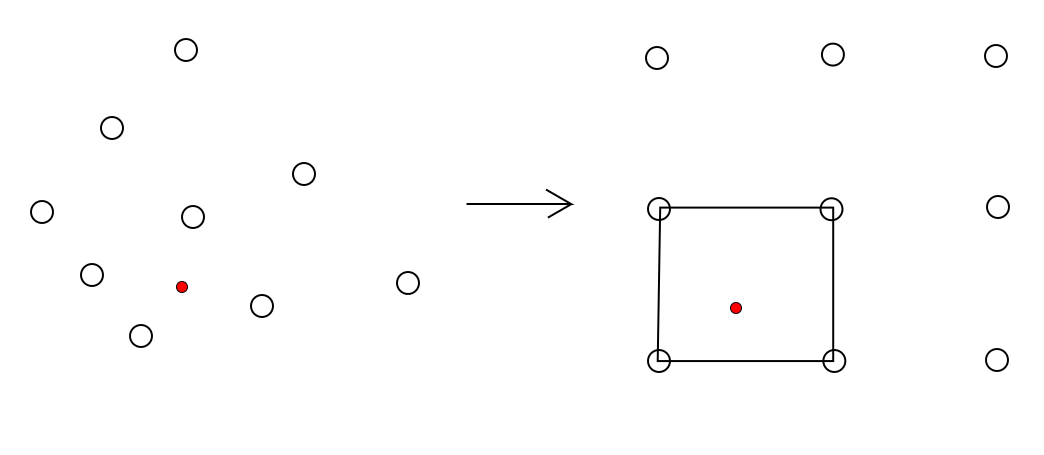
\includegraphics[width=0.8\linewidth]{figures/A1_uncertainty-analysis/interp}
\caption{}
\label{fig:interp}
\end{figure}

\chapter{GPOPS-2 Example - Brachistochrone Problem}
This section describes a short example of an optimal control problem solved in GPOPS-II. The purpose of this example is to demonstrate the effectiveness of the pseudospectral method and GPOPS-II, and to provide a simple example case to establish the terminology of an optimal control problem.  


The brachistochrone (from the Greek for 'shortest time') problem is a simple optimal control problem, which describes a ball rolling in two dimensions under gravity. The objective is to find the curve of descent which will minimise the time from point \textit{a}, where the ball is at rest, to point \textit{b}. It is assumed that gravity is constant and that there is no forces other than gravity acting on the ball. 
The analytical solution of this problem can be computed using the Euler-Lagrange equation as the equations describing a cycloid:

$x = A(\theta + \sin\theta) $,

$y=A(1 - \cos\theta)$

This problem is included within GPOPS-2 as an example problem, and has been solved to illustrate the GPOPS-2 solution set-up[cite Gpops XX]. Table XX describes the set-up of the optimal control problem in GPOPS-2. The dynamic equations for the Brachistochrone problem are:

$\dot{x} = v*cos(u)$,

$\dot{y} = v*sin(u)$,

$\dot{v} = g*sin(u)$.

\noindent These equations are provided to GPOPS-2 as the time-variant system model in this form. The control variable is set to be the descent angle. The initial constraints are defined to initiate the ball at rest at the origin, and the terminal constraints are defined to terminate the problem at coordinates of XX XX. The cost is set to minimum time, so that the solution will be the descent angle which minimises the time to get from the initial position, to the end position. 

\begin{table}
	\centering
	\begin{tabular}{|c|c|}
		\hline Primal Variables  & x Position\\& y Position\\& Velocity\\ 
		\hline Control Variables  & Angle of Descent\\ 
		\hline Initial Constraints  & Velocity\\ & x Position\\ & y Position\\
		\hline Terminal Constraints &  x Position\\ & y Position\\
		\hline Path Constraints & None \\ 
		\hline Target Cost & Minimum Time \\ 
		\hline 
	\end{tabular} 
\end{table}


The GPOPS-2 solution to the Brachistochrone problem is shown in Figure \ref{fig:Brachistochrone}, matching the analytical solution almost exactly. This is expected in this case, as the dynamics of the basic Brachistochrone problem are very simple. As the dynamics become more complex, it is no longer possible to obtain an analytical solution. For more complex problems, various methods must be used to verify the optimal solution. These methods are outlined later in this chapter, in Section XX.  

\begin{figure}[ht]
	\centering
	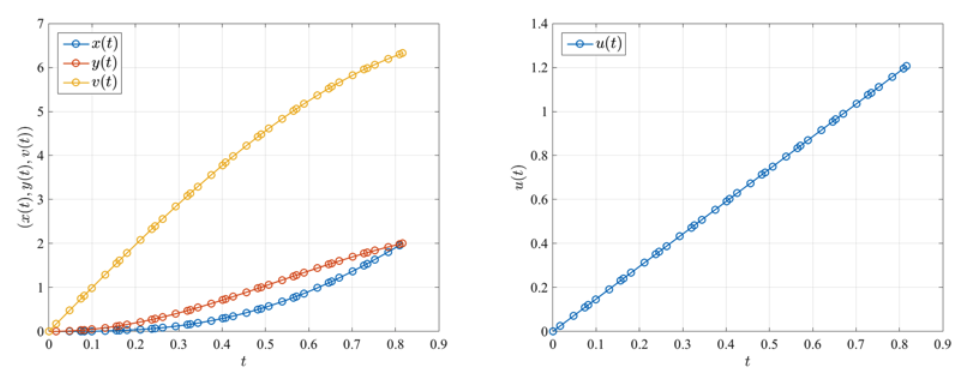
\includegraphics[width=0.9\linewidth]{figures/4_LODESTAR/Brachistochrone}
	\caption{The solution to the brachistochrone problem, solved in GPOPS-2[CITATIONXX].}
	\label{fig:Brachistochrone}
\end{figure}










\chapter{CART3D Results}

\section{Engine-On Plume Check}
-simulate engine-on conditions to check that the plumes do not adversely affect the tail of the vehicle (justify that I can just remove engines/boattail)

-Mach 5,7,9 at 50kPa

\section{CART3D Results}
-include mesh here

\begin{figure}
	\centering
	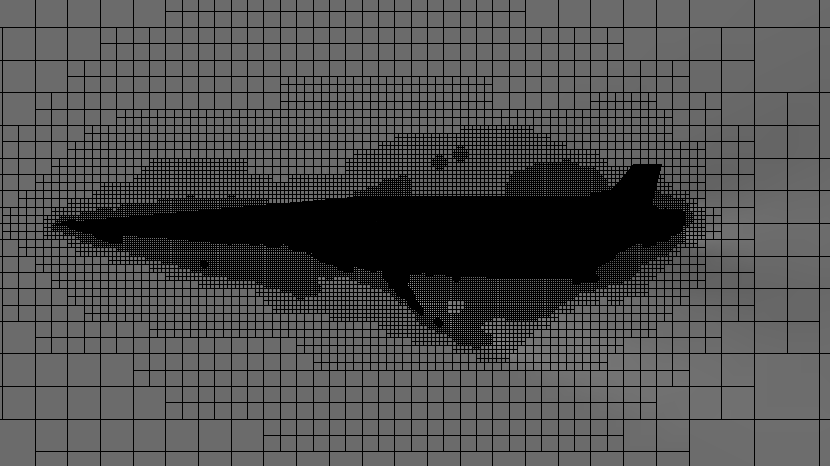
\includegraphics[width=0.7\linewidth]{figures/3_vehicle_design/M3AoA6GRID}
	\caption{}
	\label{fig:M3AoA6GRID}
\end{figure}

		\begin{figure}
			\centering
			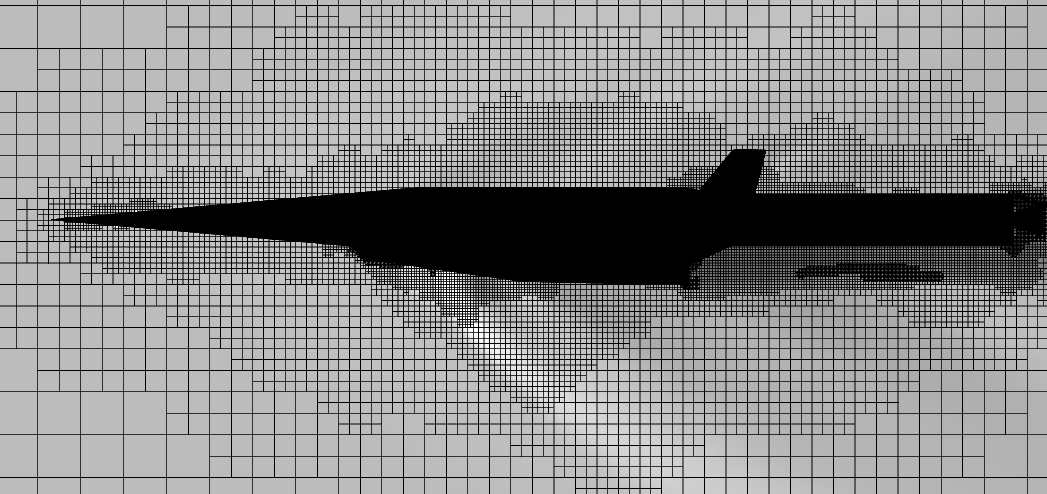
\includegraphics[width=0.7\linewidth]{figures/3_vehicle_design/CARTmesh}
			\caption{ Mesh generated by CART3D around the SPARTAN and first stage vehicles.}
			\label{fig:CARTmesh}
		\end{figure}
		
		
		
		\begin{figure}
			\centering
			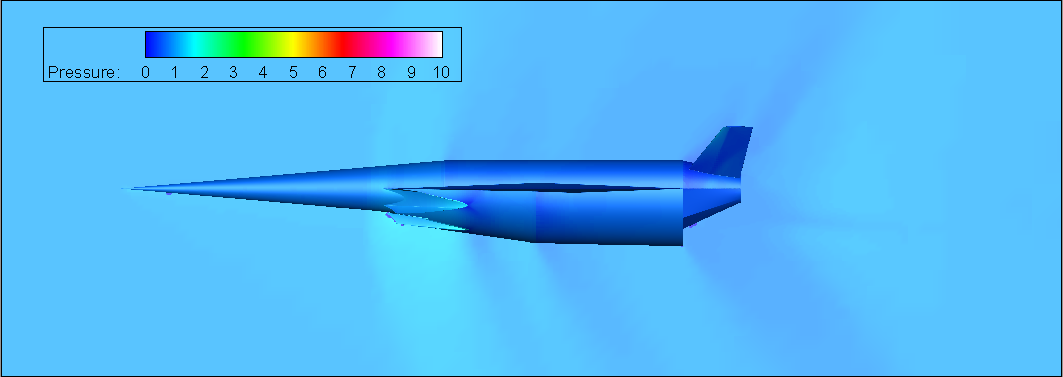
\includegraphics[width=0.9\linewidth]{figures/3_vehicle_design/M1p1AoA6}
			\caption{CART3D flow result for the SPARTAN, at Mach 1.1, 6$^\circ$ angle of attack.}
			\label{fig:M1}
		\end{figure}
		\begin{figure}
			\centering
			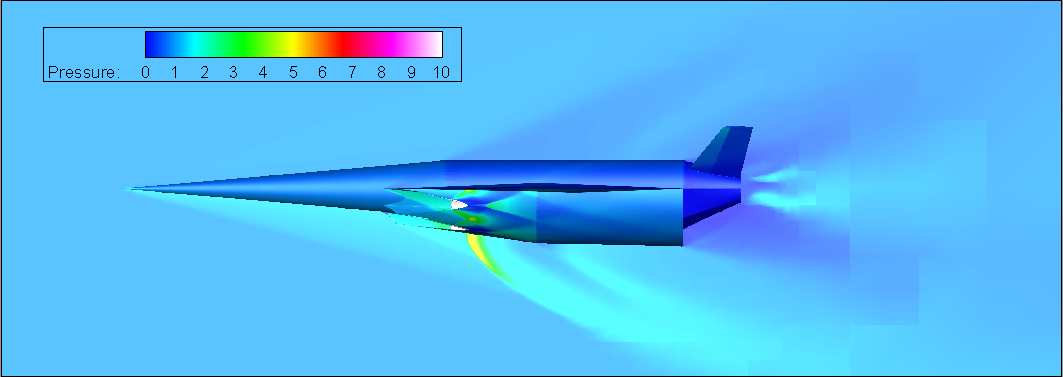
\includegraphics[width=0.9\linewidth]{figures/3_vehicle_design/M3AoA6}
			\caption{CART3D flow result for the SPARTAN, at Mach 3, 6$^\circ$ angle of attack.}
			\label{fig:M3AoA6}
		\end{figure}
		
		
		
		
		\chapter{Initial Guesses}
		
		\chapter{Optimised Trajectory Analysis}
		
		
		\section{First Stage}\label{sec:appendix_firststage}
\begin{figure}[ht!]
	\centering
	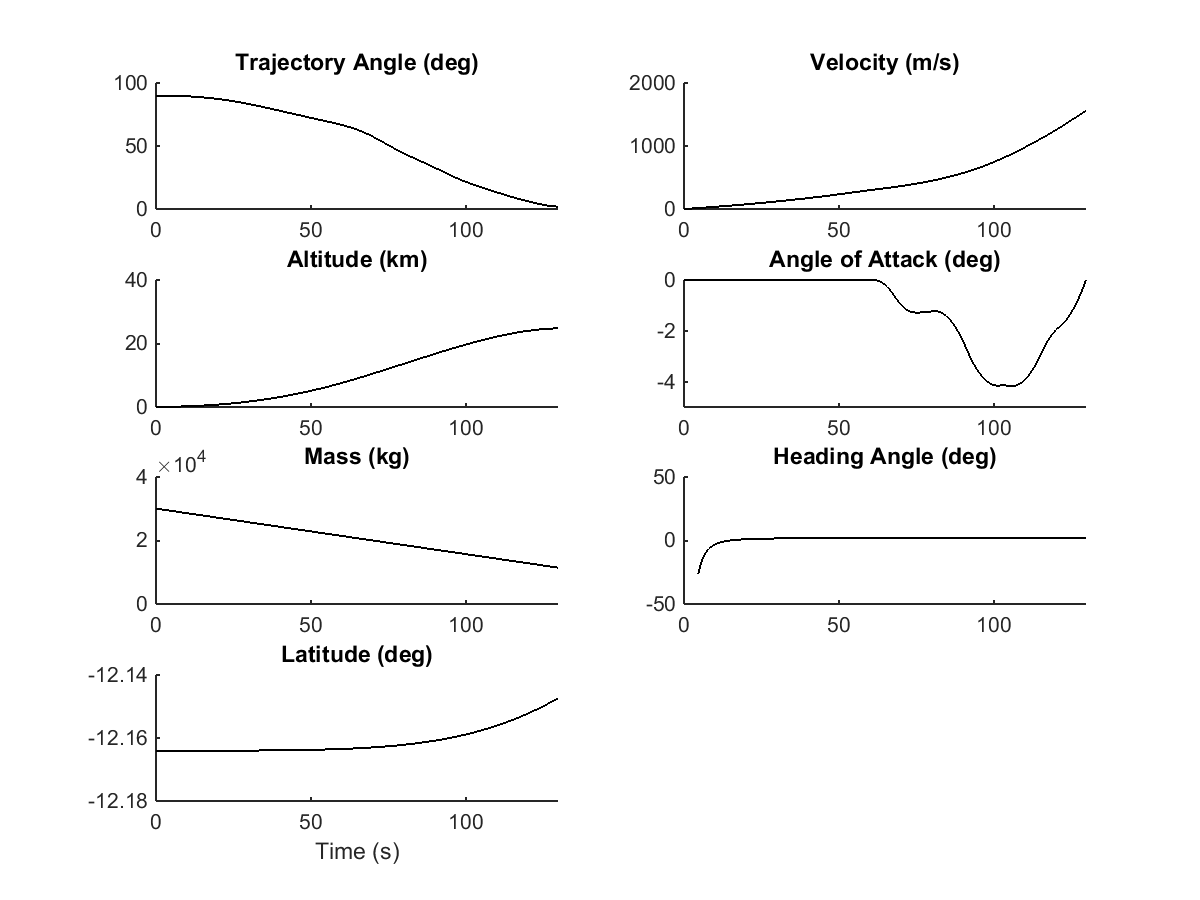
\includegraphics[width=1\linewidth]{../LODESTAR_FINAL/Results/mode11/FirstStageStandard}
	\caption{}
	\label{fig:FirstStageStandard}
\end{figure}
		
		\section{Performance History}
		
		
		\section{Verification}
		\begin{figure}
			\centering
			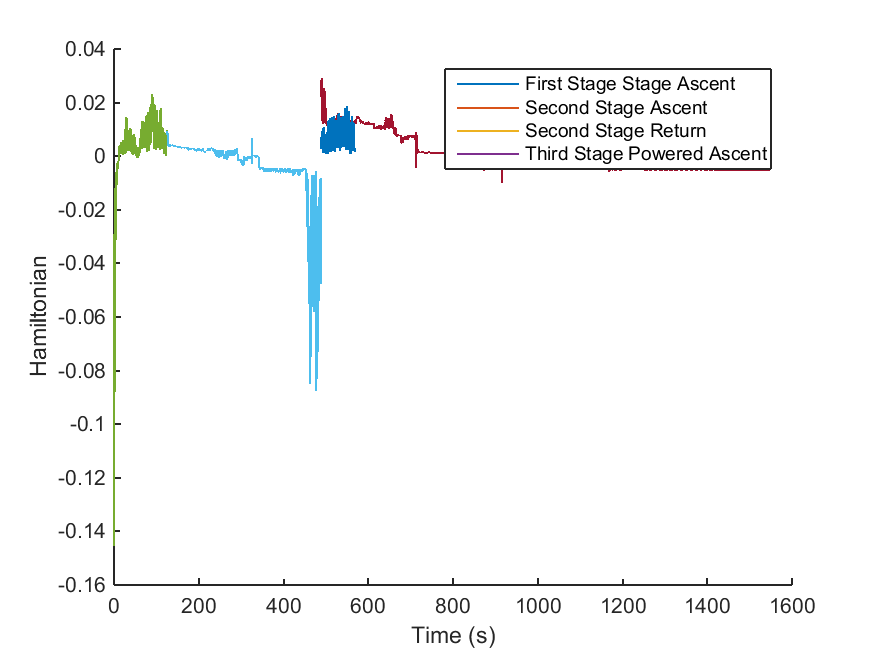
\includegraphics[width=0.7\linewidth]{../LODESTAR_FINAL/Results/mode11/HamiltonianStandard}
			\caption{}
			\label{fig:HamiltonianStandard}
		\end{figure}
		
		\begin{figure}
			\centering
			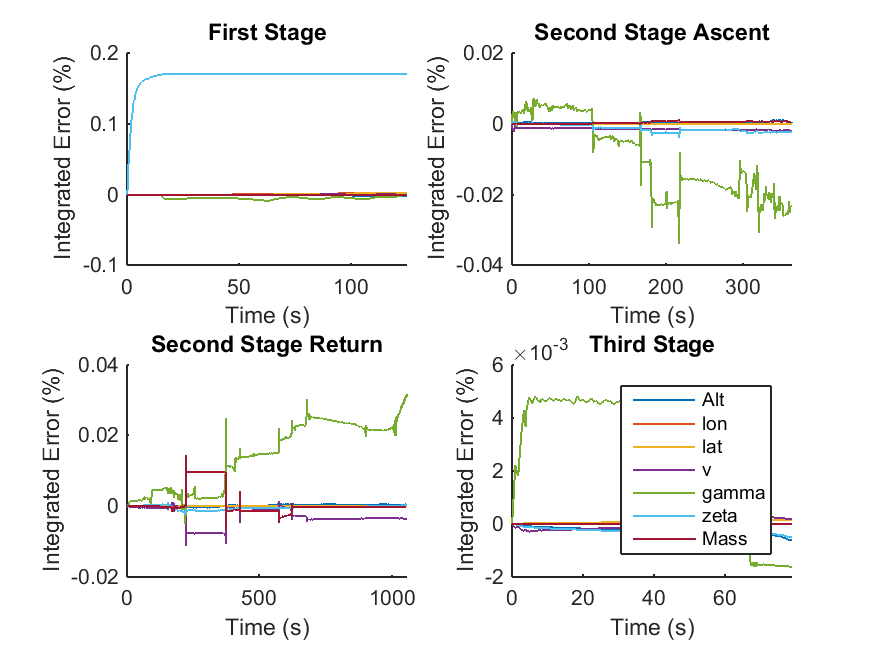
\includegraphics[width=0.7\linewidth]{../LODESTAR_FINAL/Results/mode11/VerificationStandard}
			\caption{}
			\label{fig:VerificationStandard}
		\end{figure}
		
		\begin{figure}
			\centering
			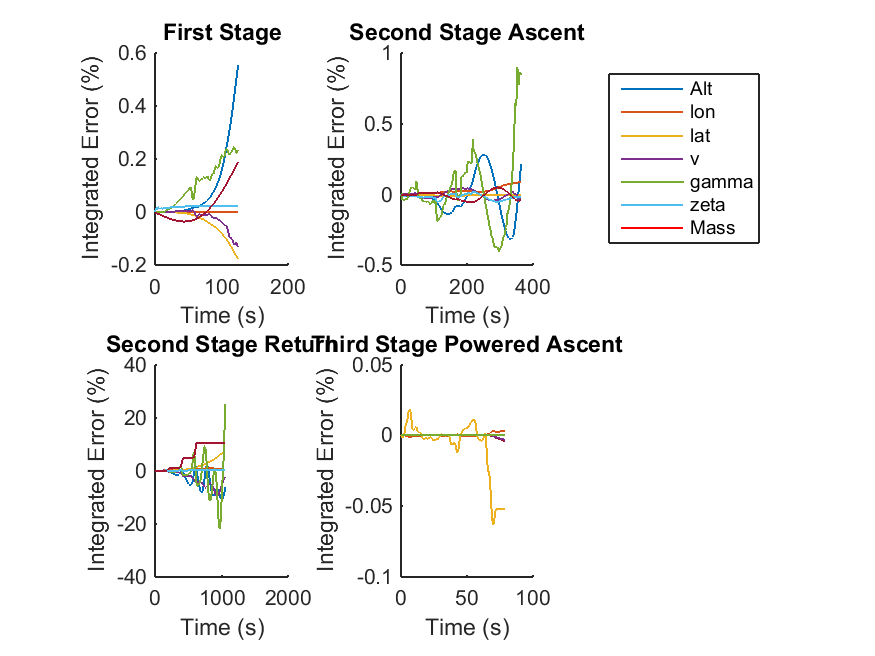
\includegraphics[width=0.7\linewidth]{../LODESTAR_FINAL/Results/mode11/ForwardErrorStandard}
			\caption{}
			\label{fig:ForwardErrorStandard}
		\end{figure}
		
		\section{Mesh History}
		
		
\begin{figure}[th]
\centering
\includegraphics[width=0.8\linewidth]{../LODESTAR_FINAL/Results/mode11/MeshHistory}
\caption{}
\label{fig:MeshHistory}
\end{figure}
		
		\chapter{Maximum Payload-To-Orbit Trajectory With Dynamic Pressure Constraint}\label{sec:Appendix_qconst}
	\begin{table}[ht]
	\centering
	\begin{tabular}{l c } 
		\hline \textbf{Trajectory Condition}
		& Constq

		\\
		\hline \textbf{Payload to Orbit (kg)}
		& \PayloadToOrbitqConstrained
		\\
		\textbf{Separation Alt, 1$\rightarrow$2 (km)}
		& \firstsecondSeparationAltqConstrained
		\\
		\textbf{Separation v, 1$\rightarrow$2 (m/s)}
		& \firstsecondSeparationvqConstrained
		\\
		\textbf{Separation $\gamma$, 1$\rightarrow$2 (m/s)}
		& \firstsecondSeparationgammaqConstrained
		\\
		\textbf{Separation Alt, 2$\rightarrow$3 (km)}
		& \secondthirdSeparationAltqConstrained
		\\
		\textbf{Separation $v$, 2$\rightarrow$3 (m/s)}
		& \secondthirdSeparationvqConstrained
		\\
		\textbf{Separation $\gamma$, 2$\rightarrow$3 (deg)}
		& \secondthirdSeparationgammaqConstrained
		\\
		\textbf{Separation $q$, 2$\rightarrow$3(kPa)}
		& \secondthirdSeparationqqConstrained
		\\
		\textbf{2$^{nd}$ Stage L/D, 2$\rightarrow$3}
		& \secondthirdSeparationLDqConstrained
		\\
		\textbf{2$^{nd}$ Stage Flight Time (s)}
		& \secondFlightTimeqConstrained
		\\
		\textbf{3$^{rd}$ Stage $t$, $q >$ 5kpa (s)}
		& \thirdqOverFiveqConstrained
		\\
		\textbf{3$^{rd}$ Stage max $\alpha$ (deg)}
		& \thirdmaxAoAqConstrained
		\\
		\textbf{3$^{rd}$ Stage final v (m/s)}
		& \thirdcircvqConstrained
		\\
		\textbf{3$^{rd}$ Stage final m (kg)}
		& \thirdcircmqConstrained
		\\
		\hline 
	\end{tabular} 
	\end{table}
		
\begin{figure}[th]
\centering
\includegraphics[width=0.8\linewidth]{../LODESTAR_FINAL/Results/10-qconstrained/FirstStageConstq}
\caption{}
\label{fig:FirstStageqConstrained68}
\end{figure}
		
\begin{figure}[th]
\centering
\includegraphics[width=0.8\linewidth]{../LODESTAR_FINAL/Results/10-qconstrained/SecondStageConstq}
\caption{}
\label{fig:SecondStageqConstrained68}
\end{figure}

\begin{figure}[th]
\centering
\includegraphics[width=0.8\linewidth]{../LODESTAR_FINAL/Results/10-qconstrained/ThirdStageConstq}
\caption{}
\label{fig:ThirdStageqConstrained68}
\end{figure}



		
		\chapter{Trajectory Plot Comparisons}\label{sec:Appendix_trajectorycomparisons}
		
		
		\section{Cases With No Fly-Back}
		
		\subsection{Dynamic Pressure Variation}
		
		
\begin{figure}[!ht]
\centering
\includegraphics[width=0.8\linewidth]{../LODESTAR_FINAL/Results/mode20/SecondStageComparison}
\caption{}
\label{fig:SecondStageComparison1}
\end{figure}

\begin{figure}[!th]
\centering
\includegraphics[width=0.8\linewidth]{../LODESTAR_FINAL/Results/mode20/ThirdStageComparison}
\caption{}
\label{fig:ThirdStageComparison1}
\end{figure}
\FloatBarrier
\subsection{Specific Impulse}


\begin{figure}[!th]
\centering
\includegraphics[width=0.8\linewidth]{../LODESTAR_FINAL/Results/mode30/SecondStageComparison}
\caption{}
\label{fig:SecondStageComparison2}

\end{figure}
\begin{figure}[!th]
\centering
\includegraphics[width=0.8\linewidth]{../LODESTAR_FINAL/Results/mode30/ThirdStageComparison}
\caption{}
\label{fig:ThirdStageComparison2}
\end{figure}
\FloatBarrier
\subsection{Drag}

\begin{figure}[!th]
\centering
\includegraphics[width=0.8\linewidth]{../LODESTAR_FINAL/Results/mode40/SecondStageComparison}
\caption{}
\label{fig:SecondStageComparison3}
\end{figure}

\begin{figure}[!th]
\centering
\includegraphics[width=0.8\linewidth]{../LODESTAR_FINAL/Results/mode40/ThirdStageComparison}
\caption{}
\label{fig:ThirdStageComparison3}
\end{figure}
\FloatBarrier
\subsection{SPARTAN Mass}

\begin{figure}[th]
\centering
\includegraphics[width=0.8\linewidth]{../LODESTAR_FINAL/Results/mode100/SecondStageComparison}
\caption{}
\label{fig:SecondStageComparison4}
\end{figure}

\begin{figure}[th]
\centering
\includegraphics[width=0.8\linewidth]{../LODESTAR_FINAL/Results/mode100/ThirdStageComparison}
\caption{}
\label{fig:ThirdStageComparison4}
\end{figure}
\FloatBarrier
\subsection{Fuel Mass}
\begin{figure}[th]
\centering
\includegraphics[width=0.8\linewidth]{../LODESTAR_FINAL/Results/mode110/SecondStageComparison}
\caption{}
\label{fig:SecondStageComparison5}
\end{figure}

\begin{figure}[th]
\centering
\includegraphics[width=0.8\linewidth]{../LODESTAR_FINAL/Results/mode110/ThirdStageComparison}
\caption{}
\label{fig:ThirdStageComparison5}
\end{figure}
\FloatBarrier
\subsection{Third Stage Mass}

\begin{figure}[th]
\centering
\includegraphics[width=0.8\linewidth]{../LODESTAR_FINAL/Results/mode80/SecondStageComparison}
\caption{}
\label{fig:SecondStageComparison6}
\end{figure}


\begin{figure}[th]
\centering
\includegraphics[width=0.8\linewidth]{../LODESTAR_FINAL/Results/mode80/ThirdStageComparison}
\caption{}
\label{fig:ThirdStageComparison6}
\end{figure}

\FloatBarrier
\subsection{Third Stage Thrust}

\begin{figure}[th]
	\centering
	\includegraphics[width=0.8\linewidth]{../LODESTAR_FINAL/Results/mode90/SecondStageComparison}
	\caption{}
	\label{fig:SecondStageComparison7}
\end{figure}

\begin{figure}[th]
\centering
\includegraphics[width=0.8\linewidth]{../LODESTAR_FINAL/Results/mode90/ThirdStageComparison}
\caption{}
\label{fig:ThirdStageComparison7}
\end{figure}
\FloatBarrier
\subsection{Third Stage Drag}

\begin{figure}[th]
\centering
\includegraphics[width=0.8\linewidth]{../LODESTAR_FINAL/Results/mode70/SecondStageComparison}
\caption{}
\label{fig:SecondStageComparison8}
\end{figure}


\begin{figure}[th]
\centering
\includegraphics[width=0.8\linewidth]{../LODESTAR_FINAL/Results/mode70/ThirdStageComparison}
\caption{}
\label{fig:ThirdStageComparison8}
\end{figure}


\section{Cases With Fly-Back}

\subsection{Dynamic Pressure Variation}
\begin{figure}[th]
\centering
\includegraphics[width=0.8\linewidth]{../LODESTAR_FINAL/Results/mode21/SecondStageComparison}
\caption{}
\label{fig:SecondStageComparison9}
\end{figure}

\begin{figure}[th]
\centering
\includegraphics[width=0.8\linewidth]{../LODESTAR_FINAL/Results/mode21/ThirdStageComparison}
\caption{}
\label{fig:ThirdStageComparison9}
\end{figure}

\begin{figure}[th]
\centering
\includegraphics[width=0.8\linewidth]{../LODESTAR_FINAL/Results/mode21/ReturnComparison}
\caption{}
\label{fig:ReturnComparison}
\end{figure}


\subsection{Specific Impulse}
\begin{figure}[th]
\centering
\includegraphics[width=0.8\linewidth]{../LODESTAR_FINAL/Results/mode31/SecondStageComparison}
\caption{}
\label{fig:SecondStageComparison10}
\end{figure}

\begin{figure}[th]
\centering
\includegraphics[width=0.8\linewidth]{../LODESTAR_FINAL/Results/mode31/ThirdStageComparison}
\caption{}
\label{fig:ThirdStageComparison10}
\end{figure}

\begin{figure}[th]
\centering
\includegraphics[width=0.8\linewidth]{../LODESTAR_FINAL/Results/mode31/ReturnComparison}
\caption{}
\label{fig:ReturnComparison10}
\end{figure}


\subsection{Drag}
\begin{figure}[th]
\centering
\includegraphics[width=0.8\linewidth]{../LODESTAR_FINAL/Results/mode41/SecondStageComparison}
\caption{}
\label{fig:SecondStageComparison11}
\end{figure}

\begin{figure}[th]
\centering
\includegraphics[width=0.8\linewidth]{../LODESTAR_FINAL/Results/mode41/ThirdStageComparison}
\caption{}
\label{fig:ThirdStageComparison11}
\end{figure}

\begin{figure}[th]
\centering
\includegraphics[width=0.8\linewidth]{../LODESTAR_FINAL/Results/mode41/ReturnComparison}
\caption{}
\label{fig:ReturnComparison11}
\end{figure}


\subsection{SPARTAN Mass}

\begin{figure}[th]
\centering
\includegraphics[width=0.8\linewidth]{../LODESTAR_FINAL/Results/mode101/SecondStageComparison}
\caption{}
\label{fig:SecondStageComparison12}
\end{figure}

\begin{figure}[th]
\centering
\includegraphics[width=0.8\linewidth]{../LODESTAR_FINAL/Results/mode101/ThirdStageComparison}
\caption{}
\label{fig:ThirdStageComparison12}
\end{figure}

\begin{figure}[th]
\centering
\includegraphics[width=0.8\linewidth]{../LODESTAR_FINAL/Results/mode101/ReturnComparison}
\caption{}
\label{fig:ReturnComparison12}
\end{figure}


\subsection{Fuel Mass}

\begin{figure}[th]
\centering
\includegraphics[width=0.8\linewidth]{../LODESTAR_FINAL/Results/mode111/SecondStageComparison}
\caption{}
\label{fig:SecondStageComparison13}
\end{figure}

\begin{figure}[th]
\centering
\includegraphics[width=0.8\linewidth]{../LODESTAR_FINAL/Results/mode111/ThirdStageComparison}
\caption{}
\label{fig:ThirdStageComparison13}
\end{figure}

\begin{figure}[th]
\centering
\includegraphics[width=0.8\linewidth]{../LODESTAR_FINAL/Results/mode111/ReturnComparison}
\caption{}
\label{fig:ReturnComparison13}
\end{figure}



\subsection{Third Stage Mass}
\begin{figure}[th]
\centering
\includegraphics[width=0.8\linewidth]{../LODESTAR_FINAL/Results/mode81/SecondStageComparison}
\caption{}
\label{fig:SecondStageComparison14}
\end{figure}

\begin{figure}[th]
\centering
\includegraphics[width=0.8\linewidth]{../LODESTAR_FINAL/Results/mode81/ThirdStageComparison}
\caption{}
\label{fig:ThirdStageComparison14}
\end{figure}



\begin{figure}[th]
	\centering
	\includegraphics[width=0.8\linewidth]{../LODESTAR_FINAL/Results/mode81/ReturnComparison}
	\caption{}
	\label{fig:ReturnComparison14}
\end{figure}

\subsection{Third Stage Thrust}

\begin{figure}[th]
\centering
\includegraphics[width=0.8\linewidth]{../LODESTAR_FINAL/Results/mode91/SecondStageComparison}
\caption{}
\label{fig:SecondStageComparison15}
\end{figure}


\begin{figure}[th]
\centering
\includegraphics[width=0.8\linewidth]{../LODESTAR_FINAL/Results/mode91/ThirdStageComparison}
\caption{}
\label{fig:ThirdStageComparison15}
\end{figure}


\begin{figure}[th]
\centering
\includegraphics[width=0.8\linewidth]{../LODESTAR_FINAL/Results/mode91/ReturnComparison}
\caption{}
\label{fig:ReturnComparison15}
\end{figure}


\chapter{Viscous Drag Variation}


The viscous drag component of the SPARTAN's aerodynamics is calculated using flat plate correlations, which require an estimation of the laminar to turbulent transition point on the body of the SPARTAN[CITEXX]. This transition point is difficult to estimate to a high degree of accuracy without prohibitively time consuming CFD, and can have a significant effect on the viscous drag of an aircraft[CITEXX].
The viscous drag component of the SPARTAN's aerodynamics is varied, in order to assess the impact of the viscous drag model used. Optimal trajectories are calculated with the viscous drag set at levels of 20\%, 50\%, 107\% and 115\% of the baseline, which correspond to the possible viscous drag range due to transition point variation.

\textcolor{red}{note: regression doesnt work for this} 
\begin{table}[ht]
	\centering
	\begin{tabular}{l c c c c c c} 
		\hline \textbf{Trajectory Condition}
		&vCdTwenty
		&vCdFifty
		&vCdStandard
		&vCdOneHundredSeven
		&vCdOneHundredFifteen
		& /\%
		\\
		\hline \textbf{Payload to Orbit (kg)}
		& \PayloadToOrbitvCdTwenty
		& \PayloadToOrbitvCdFifty
		& \PayloadToOrbitvCdStandard
		& \PayloadToOrbitvCdOneHundredSeven
		& \PayloadToOrbitvCdOneHundredFifteen
		&-2.5
		\\
		\textbf{Separation Alt, 1$\rightarrow$2 (km)}
		& \firstsecondSeparationAltvCdTwenty
		& \firstsecondSeparationAltvCdFifty
		& \firstsecondSeparationAltvCdStandard
		& \firstsecondSeparationAltvCdOneHundredSeven
		& \firstsecondSeparationAltvCdOneHundredFifteen
		& -
		\\
		\textbf{Separation v, 1$\rightarrow$2 (m/s)}
		& \firstsecondSeparationvvCdTwenty
		& \firstsecondSeparationvvCdFifty
		& \firstsecondSeparationvvCdStandard
		& \firstsecondSeparationvvCdOneHundredSeven
		& \firstsecondSeparationvvCdOneHundredFifteen
		& -
		\\
		\textbf{Separation $\gamma$, 1$\rightarrow$2 (m/s)}
		& \firstsecondSeparationgammavCdTwenty
		& \firstsecondSeparationgammavCdFifty
		& \firstsecondSeparationgammavCdStandard
		& \firstsecondSeparationgammavCdOneHundredSeven
		& \firstsecondSeparationgammavCdOneHundredFifteen
		& -
		\\
		\textbf{Separation Alt, 2$\rightarrow$3 (km)}
		& \secondthirdSeparationAltvCdTwenty
		& \secondthirdSeparationAltvCdFifty
		& \secondthirdSeparationAltvCdStandard
		& \secondthirdSeparationAltvCdOneHundredSeven
		& \secondthirdSeparationAltvCdOneHundredFifteen
		& -
		\\
		\textbf{Separation $v$, 2$\rightarrow$3 (m/s)}
		& \secondthirdSeparationvvCdTwenty
		& \secondthirdSeparationvvCdFifty
		& \secondthirdSeparationvvCdStandard
		& \secondthirdSeparationvvCdOneHundredSeven
		& \secondthirdSeparationvvCdOneHundredFifteen
		&-33.89
		\\
		\textbf{Separation $\gamma$, 2$\rightarrow$3 (deg)}
		& \secondthirdSeparationgammavCdTwenty
		& \secondthirdSeparationgammavCdFifty
		& \secondthirdSeparationgammavCdStandard
		& \secondthirdSeparationgammavCdOneHundredSeven
		& \secondthirdSeparationgammavCdOneHundredFifteen
		&-0.1
		\\
		\textbf{Separation $q$, 2$\rightarrow$3(kPa)}
		& \secondthirdSeparationqvCdTwenty
		& \secondthirdSeparationqvCdFifty
		& \secondthirdSeparationqvCdStandard
		& \secondthirdSeparationqvCdOneHundredSeven
		& \secondthirdSeparationqvCdOneHundredFifteen
		&-0.16
		\\
		\textbf{2$^{nd}$ Stage L/D, 2$\rightarrow$3}
		& \secondthirdSeparationLDvCdTwenty
		& \secondthirdSeparationLDvCdFifty
		& \secondthirdSeparationLDvCdStandard
		& \secondthirdSeparationLDvCdOneHundredSeven
		& \secondthirdSeparationLDvCdOneHundredFifteen
		& -
		\\
		\textbf{2$^{nd}$ Stage Flight Time (s)}
		& \secondFlightTimevCdTwenty
		& \secondFlightTimevCdFifty
		& \secondFlightTimevCdStandard
		& \secondFlightTimevCdOneHundredSeven
		& \secondFlightTimevCdOneHundredFifteen
		& -
		\\
		\textbf{2$^{nd}$ Stage Return Fuel (kg)}
		& \returnFuelvCdTwenty
		& \returnFuelvCdFifty
		& \returnFuelvCdStandard
		& \returnFuelvCdOneHundredSeven
		& \returnFuelvCdOneHundredFifteen
		& -
		\\
		\textbf{3$^{rd}$ Stage $t$, $q >$ 5kpa (s)}
		& \thirdqOverFivevCdTwenty
		& \thirdqOverFivevCdFifty
		& \thirdqOverFivevCdStandard
		& \thirdqOverFivevCdOneHundredSeven
		& \thirdqOverFivevCdOneHundredFifteen
		&-0.22
		\\
		\textbf{3$^{rd}$ Stage max $\alpha$ (deg)}
		& \thirdmaxAoAvCdTwenty
		& \thirdmaxAoAvCdFifty
		& \thirdmaxAoAvCdStandard
		& \thirdmaxAoAvCdOneHundredSeven
		& \thirdmaxAoAvCdOneHundredFifteen
		& -
		\\
		\textbf{3$^{rd}$ Stage final v (m/s)}
		& \thirdcircvvCdTwenty
		& \thirdcircvvCdFifty
		& \thirdcircvvCdStandard
		& \thirdcircvvCdOneHundredSeven
		& \thirdcircvvCdOneHundredFifteen
		&-47.52
		\\
		\textbf{3$^{rd}$ Stage final m (kg)}
		& \thirdcircmvCdTwenty
		& \thirdcircmvCdFifty
		& \thirdcircmvCdStandard
		& \thirdcircmvCdOneHundredSeven
		& \thirdcircmvCdOneHundredFifteen
		& -
		\\
		\hline 
	\end{tabular} 
\end{table} 

\subsubsection{Trajectory Comparisons}
\begin{figure}[th]
\centering
\includegraphics[width=0.8\linewidth]{../LODESTAR_FINAL/Results/mode51/SecondStageComparison}
\caption{}
\label{fig:SecondStageComparison-}
\end{figure}
\begin{figure}[th]
\centering
\includegraphics[width=0.8\linewidth]{../LODESTAR_FINAL/Results/mode51/ThirdStageComparison}
\caption{}
\label{fig:ThirdStageComparison-}
\end{figure}


\begin{figure}[th]
	\centering
	\includegraphics[width=0.8\linewidth]{../LODESTAR_FINAL/Results/mode51/ReturnComparison}
	\caption{}
	\label{fig:ReturnComparison-}
\end{figure}

\chapter{Overpressure Response Studies}

\begin{figure}[ht]
	\centering
	\includegraphics[width=0.6\linewidth]{figures/6_FlyBack/OverPressureResponse}
	\caption{\textcolor{red}{It will be make clear on this figure which areas are flying over land. }}
	\label{fig:OverPressureResponse}
\end{figure}